\newpage
\subsection{Preparation of Australian tidal solution to support regional \OGCM{}}
\label{S:plan_OTIS}

\subsubsection{Problem and motivation}
Open boundary conditions (OBC) are a fundamental to any limited area regional \OGCM{} simulation.  
Tide resolving regional simulations typically rely on OBCs derived from the combination of distinct tidal and nontidal nesting models.   Such a combination has direct analogues to the time series `aggregation' of sea level discussed previously (eg Section \ref{S:plan_insitu_analysis}).\\
On the premise that gridded harmonic tidal solutions will continue to be utilised for this purpose into the foreseeable future:
\BoxBegin{}
can a regional tidal solution be optimised for the purposes of providing open boundary conditions for an Australian regional \OGCM{}?
\BoxEnd{}

Compared to published global solutions  `better' regional tidal data may result from 
\begin{inparaenum}[(a)]
\item restricting the spatial extent of the inversion;
\item including additional observational constraints;
\item more appropriate bathymetry;
\item tuning inversion parameters.
\end{inparaenum}

Moreover, it is asserted that the ultimate use as an aggregated OBC is relevant to the preparation of the tidal solution.   The best tidal solution for use as OBC need not be identical to the best stand-alone regional tide model.\\
Thus the details of how the \OGCM{} treats the tidal OBC are relevant considerations.  A regional configuration of \MOM{} (e.g.. \OFAMHR{}) is currently planned to be used as the reference in this regard; however, \ROMS{} is flagged as a alternative that may ultimately be considered more relevant.



\subsubsection{Data sources}
Latest TPX - global OBC for the tidal forward model.
Altimetry 
Select tidal constituents produced for the ANTT.
OTIS.


\subsubsection{Method outlook}
This work will be centred on use of the Oregon State University Tidal Inversion Software (\OTIS{}) tools and procedures \cite{Egbert:2002ug}.\\
Detailed consideration of the \OTIS{} inversion process with regard to the ultimate use as an OBC will form the body of this investigation.   Aspects to be addressed include:
\begin{itemize}
\item compatibility of the \OTIS{} forward tide model with the \OGCM{};
\item trade-off between elevation and transport constraints;
\item spatial design of the observational dataset;
\item constituent selection, covariances and inference;
\end{itemize}

For clarity, a distinction is noted between the inversion software itself and distributed solutions derived from it - both of which are commonly referred to as \OTIS{}.  To date, basic proficiency with the \OTIS{} inversion process and some trial solutions have been developed.  The relevance of an international study trip that involved discussions with the software developers and experts is noted also.

\begin{figure}[h]
\begin{center}
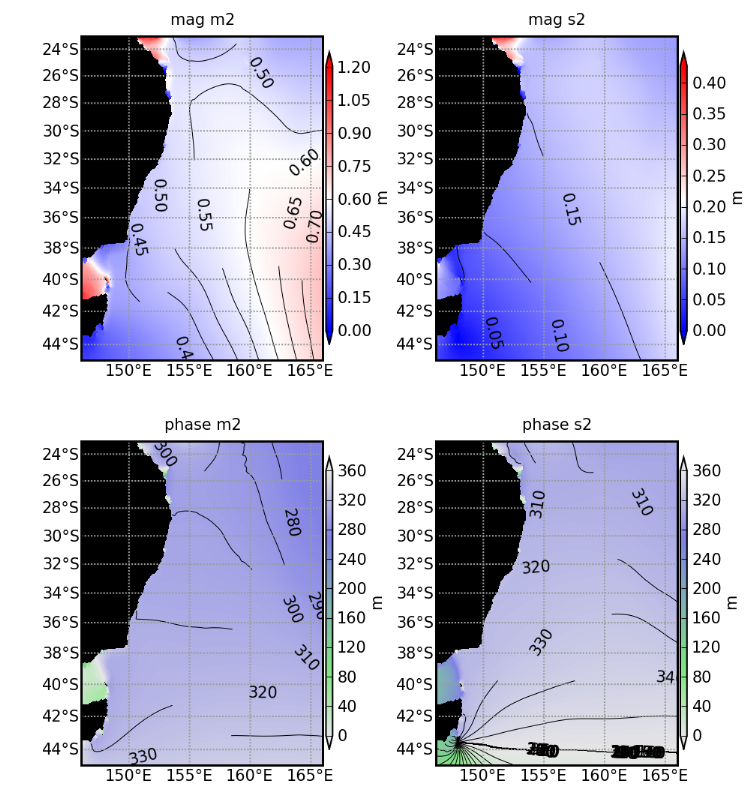
\includegraphics[width=100mm]{figures_3/otis_example.png}
\caption{Illustration of trials to implement tidal data assimilation using \OTIS{}}
\label{fig:OTIS_eg}
\end{center}
\end{figure}


The end point to this study will involve quantitative evaluation of \OGCM{} simulations carried out to assess the impact of candidate tidal solutions.









